\documentclass[border = 3mmm]{standalone}
\usepackage{pgfplots}
\usepgfplotslibrary{groupplots}
\pgfplotsset{width=10cm,compat=newest}  % <<height>>

\begin{document}

\begin{tabular}{c}
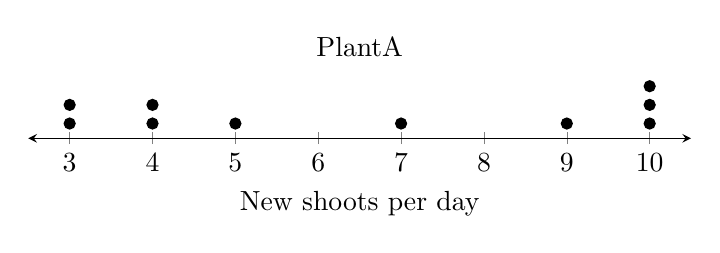
\begin{tikzpicture}
    \begin{axis}[
        height=2.15cm,
        xmin=2.5,
        xmax=10.5,
        % hide y axis,
        axis y line=none,
        axis x line=bottom,
        % set the precision of the x tick labels to be 0, which means no decimals
        % xticklabel style={/pgf/number format/precision=0},
        xtick={3,4,...,10},
        axis x line shift={4pt},
        every outer x axis line/.append style={stealth-stealth},
        title={PlantA},
        xlabel={New shoots per day}]
        \addplot [only marks, black, mark=*, mark size=2pt] coordinates{(3, 1)(3, 2)(4, 1)(4, 2)(5, 1)(7, 1)(9, 1)(10, 1)(10, 2)(10, 3)};
    \end{axis}
\end{tikzpicture}
\\
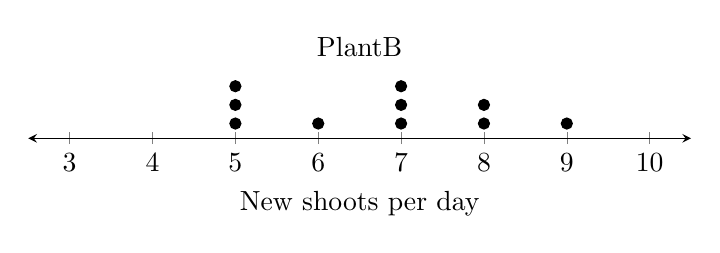
\begin{tikzpicture}
    \begin{axis}[
    height=2.15cm,
    xmin=2.5,
    xmax=10.5,
    % hide y axis,
    axis y line=none,
    axis x line=bottom,
    xtick={3,4,...,10},
    axis x line shift={4pt},
    every outer x axis line/.append style={stealth-stealth},
    mark=*,
    title={PlantB},
    xlabel={New shoots per day}]
    \addplot [only marks] coordinates{(5, 1)(5, 2)(5, 3)(6, 1)(7, 1)(7, 2)(7, 3)(8, 1)(8, 2)(9, 1)};
    \end{axis}
\end{tikzpicture}
\\
\end{tabular}

\end{document}


